\section{Exercise 1: Haar-like features and classification}

\subsection{Compute and visualize Haar-like features}

\ref{fig:integralim}

\begin{figure}[htb]
	\centering
		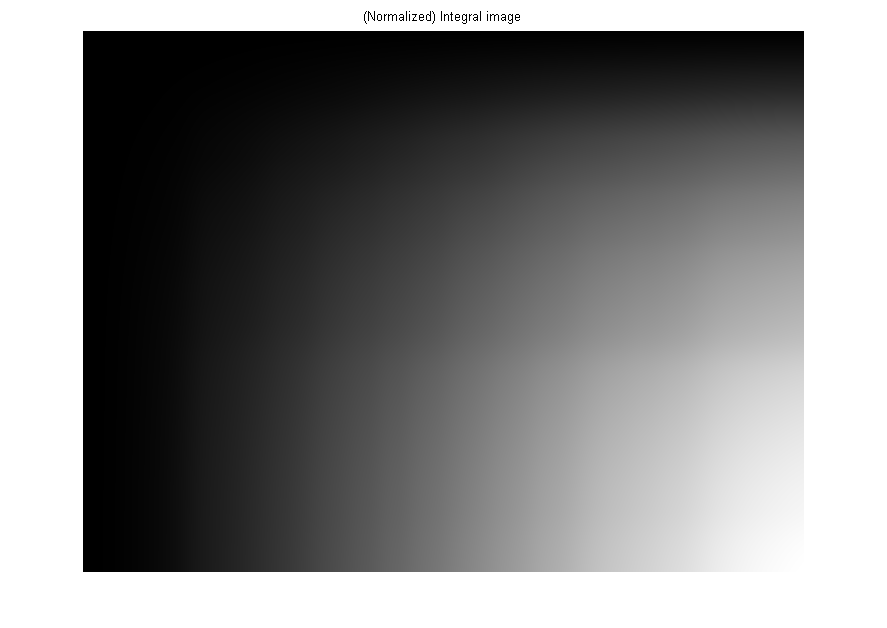
\includegraphics{./img/ex1/integralim.png}
	\caption{Integral image}
	\label{fig:integralim}
\end{figure}


{\bfseries
Question 1:
\begin{itemize}
\item Explain the obtained 2-dimensional plot on the feature space.
\item Given this 2-dimensional plot, can we infer the defined Haar-like features
			are appropriate for face/non-face discrimination?
\end{itemize}}

\subsecion{Classification in the feature space}

{\bfseries Question 2: \\Is the result good enough? Explain your response}

{\bfseries Question 3: \\What do you infer from the figure? Explain your response}